\chapter{Quantum computing} \label{Quantum computing}

\section{Introduction}
As mentioned in the introduction, quantum computers are specialized calculators which exploit the laws of quantum mechanics to perform the computations. This process is also called 'quantum computing' or 'quantum computation'. \\
A definition of quantum computation, together with quantum information, is the study of the information processing tasks that can be accomplished using quantum mechanical systems. \\
\\
The first historical strand contributing to the development of quantum computation and quantum information is the interest, dating to the 1970s, of obtaining complete control over single quantum systems. This research comprehend, for example, experiments on Bell's inequality formula and entanglement between particles. \\
This field is very important for scientific research, since it represents a method for probing a new regime of Nature of which we know so little. \\
\\
The second motivation is the intersection with the field of computer science. Since the standardization of digital computers in 1947, year in which John Bardeen, Walter Brattain, and Will Shockley developed the transistor, classical computer hardware has grown in power at an amazing pace, following the so-called Moore's law, which states that computer power will double constantly roughly once every two years. Nowadays, though conventional approaches to the fabrication of computer technology are beginning to run up against fundamental difficulties of size, quantum effects are beginning to interfere in the functioning of electronic devices as they are made smaller and smaller. \\
\\
Still, at a more fundamental level are classical and quantum computers different from one another? Notoriously, in 1936 mathematician Alan Turing developed in detail an abstract notion of what we would now call a programmable computer, a model for computation now known as the Turing machine, in his honor. Turing showed that there is a universal Turing machine that can be used to simulate any other Turing machine. Furthermore, he claimed that the universal Turing machine completely captures what it means to perform a task by algorithmic means. That is, if an algorithm can be performed on any piece of hardware, then there is an equivalent algorithm for a universal Turing machine which performs exactly the same task as the algorithm running on the personal computer. This assertion, known as the Church–Turing thesis in honor of Turing and another pioneer of computer science, Alonzo Church, asserts the equivalence between the physical concept of what class of algorithms can be performed on some physical device with the rigorous mathematical concept of a universal Turing machine. What was noticed in the late 1960s and early 1970s was that it seemed as though the Turing machine model of computation was at least as powerful as any other model of computation, in the sense that a problem which could be solved efficiently in some model of computation could also be solved efficiently in the Turing machine model, by using the Turing machine to simulate the other model of computation. This observation was codified into a strengthened version of the Church–Turing thesis:
\begin{quote}
    \textit{Any algorithmic process can be simulated efficiently using a Turing machine.}
\end{quote}
The key strengthening in the strong Church–Turing thesis is the word efficiently. Roughly speaking, an efficient algorithm is one which runs in time polynomial in the size of the problem solved. In contrast, an inefficient algorithm requires superpolynomial (typically exponential) time. If the strong Church–Turing thesis is correct, then it implies that no matter what type of machine we use to perform our algorithms, that machine can be simulated efficiently using a standard Turing machine. This is an important strengthening, as it implies that for the purposes of analyzing whether a given computational task can be accomplished efficiently, we may restrict ourselves to the analysis of the Turing machine model of computation. \\
The first major challenge to the strong Church–Turing thesis arose in the mid 1970s, when Robert Solovay and Volker Strassen showed that it is possible to test whether an integer is prime or composite using a randomized algorithm. This, together with other such algorithms brought to a modification of the strong Church–Turing thesis:
\begin{quote}
    \textit{Any algorithmic process can be simulated efficiently using a probabilistic Turing machine.}
\end{quote}
This ad hoc modification of the strong Church–Turing thesis rises many doubts. Might it not turn out at some later date that yet another model of computation allows one to efficiently solve problems that are not efficiently soluble within Turing’s model of computation? Is there any way we can find a single model of computation which is guaranteed to be able to efficiently simulate any other model of computation? \\
\\
Motivated by this question, in 1985 David Deutsch asked whether the laws of physics could be used to derive an even stronger version of the Church–Turing thesis. Because the laws of physics are ultimately quantum mechanical, Deutsch was naturally led to consider computing devices based upon the principles of quantum mechanics. These devices, quantum analogues of the machines defined forty-nine years earlier by Turing, led ultimately to the modern conception of a quantum computer. \\
It is not clear whether Deutsch’s notion of a universal quantum computer is sufficient to efficiently simulate an arbitrary physical system. Proving or refuting this conjecture is one of the great open problems of the field of quantum computation and quantum information. It is possible, for example, that some effect of quantum field theory or an even more exotic effect based in string theory, quantum gravity or some other physical theory may take us beyond Deutsch’s universal quantum computer, giving us a still more powerful model for computation. \\
What Deutsch’s model of a quantum computer did enable was a challenge to the strong form of the Church–Turing thesis. Deutsch asked whether it is possible for a quantum computer to efficiently solve computational problems which have no efficient solution on a classical computer, even a probabilistic Turing machine. He then constructed a simple example suggesting that, indeed, quantum computers might have computational powers exceeding those of classical computers. \\
\\
It turns out that while an ordinary computer can be used to simulate a quantum computer, it appears to be impossible to perform the simulation in an efficient fashion. Thus quantum computers offer an essential speed advantage over classical computers. This speed advantage is so significant that many researchers believe that no conceivable amount of progress in classical computation would be able to overcome the gap between the power of a classical computer and the power of a quantum computer. \\
The remarkable first step taken by Deutsch was in fact improved in the subsequent decade by many people, culminating in the already mentioned Peter Shor’s 1994 demonstration that the problem of finding the prime factors of an integer, and the so-called ‘discrete logarithm problem', could be solved efficiently on a quantum computer \cite{Shor1994Nov} and in 1995 when Lov Grover showed that the problem of conducting a search through some unstructured search space could also be sped up on a quantum computer \cite{Grover1996Jul}. \\
\\
More recently, many companies, among which Google, IBM and Microsoft, invested a great deal of money in research and development of this new technology. In 2019 researchers at Google claimed they achieved the so-called 'quantum supremacy' with a 53 qubits quantum processor called Sycamore, a term to describe the huge advantage a process executed on a quantum computer can reach against the same process executed on a classical computer. The process consisted in sampling the probability distribution of all the possible outputs of a pseudorandom quantum circuit, comparing them with the theoretically expected values \cite{Arute2019Oct}. \\
On the other side, IBM is among the first companies to have developed and made available quantum computers, even though with little computational power, up to tens of qubits, and plans to build more and more powerful ones in the coming years, as showed in the IBM roadmap for quantum computation (we will focus more on this topic in Chapter \ref{Computational advantage}). \\
\\
Let's now describe the fundamentals of quantum computing. \\
Classical computer circuits consist of wires and logic gates. The wires are used to carry information around the circuit, while the logic gates perform manipulations of the information, converting it from one form to another. \\
In quantum computing there are wires used to carry quantum information, i.e. qubits, and quantum logic gates, which manipulate the information. They are generally presented in a circuital form, where single lines represent qubits and parallel lines represent classical bits. \\
A collection of qubits, as well as a collection of bits, is called a register. These are the targets of the manipulation. \\
Specific simbols representing the gates are placed on the path to indicate the transformations applied to the register. \\
A quantum algorithm is an algorithm designed for a quantum computer, it can be described mathematically as a sequence of operations on quantum states or pictured in a quantum circuit, which generally end with the measurement of the states of the registers. \\
As we see there is a one-to-one correspondence between the two paradigms. This is referred to as digital quantum computing, but other type of schemes can be used to carry on the calculation, such as analog quantum computing or adiabatic quantum computing.

\subsection{Qubits}
A qubit, short for quantum bit, is the basic unit of quantum information, analogous to a bit for classical information. It is a two-state quantum system that can be described as a vector in a two dimension Hilbert space $\mathcal{H}$, whose basis vectors are pure states $|0\rangle = \left( \begin{array}{c} 1 \\ 0 \end{array} \right)$ and $|1\rangle = \left( \begin{array}{c} 0 \\ 1 \end{array} \right)$, together called the 'computational basis'. This definition derives naturally from the first postulate of quantum mechanics. \\
The state of a qubit is usually expressed as a superposition of these two basis states
\begin{equation}
    |\psi\rangle = \alpha |0\rangle + \beta |1\rangle = \left( \begin{array}{c} \alpha \\ \beta \end{array} \right), \label{qubit}
\end{equation}
where $\alpha, \beta \in \mathbb{C}$ and $|\alpha|^2 + |\beta|^2 = 1$, or in a form that exploit the normalization of the state
\begin{equation}
    |\psi\rangle = cos \frac{\theta}{2} |0\rangle + e^{i\phi} sin \frac{\theta}{2} |1\rangle,
\end{equation}
with $0 \leq \theta \leq \pi$ and $0 \leq \phi \leq 2\pi$. This last representation is called the 'Bloch sphere', because $\theta$ and $\phi$ represent the azimuthal and the polar variables of the spherical coordinate system.
\begin{figure}[ht]
  \centering
  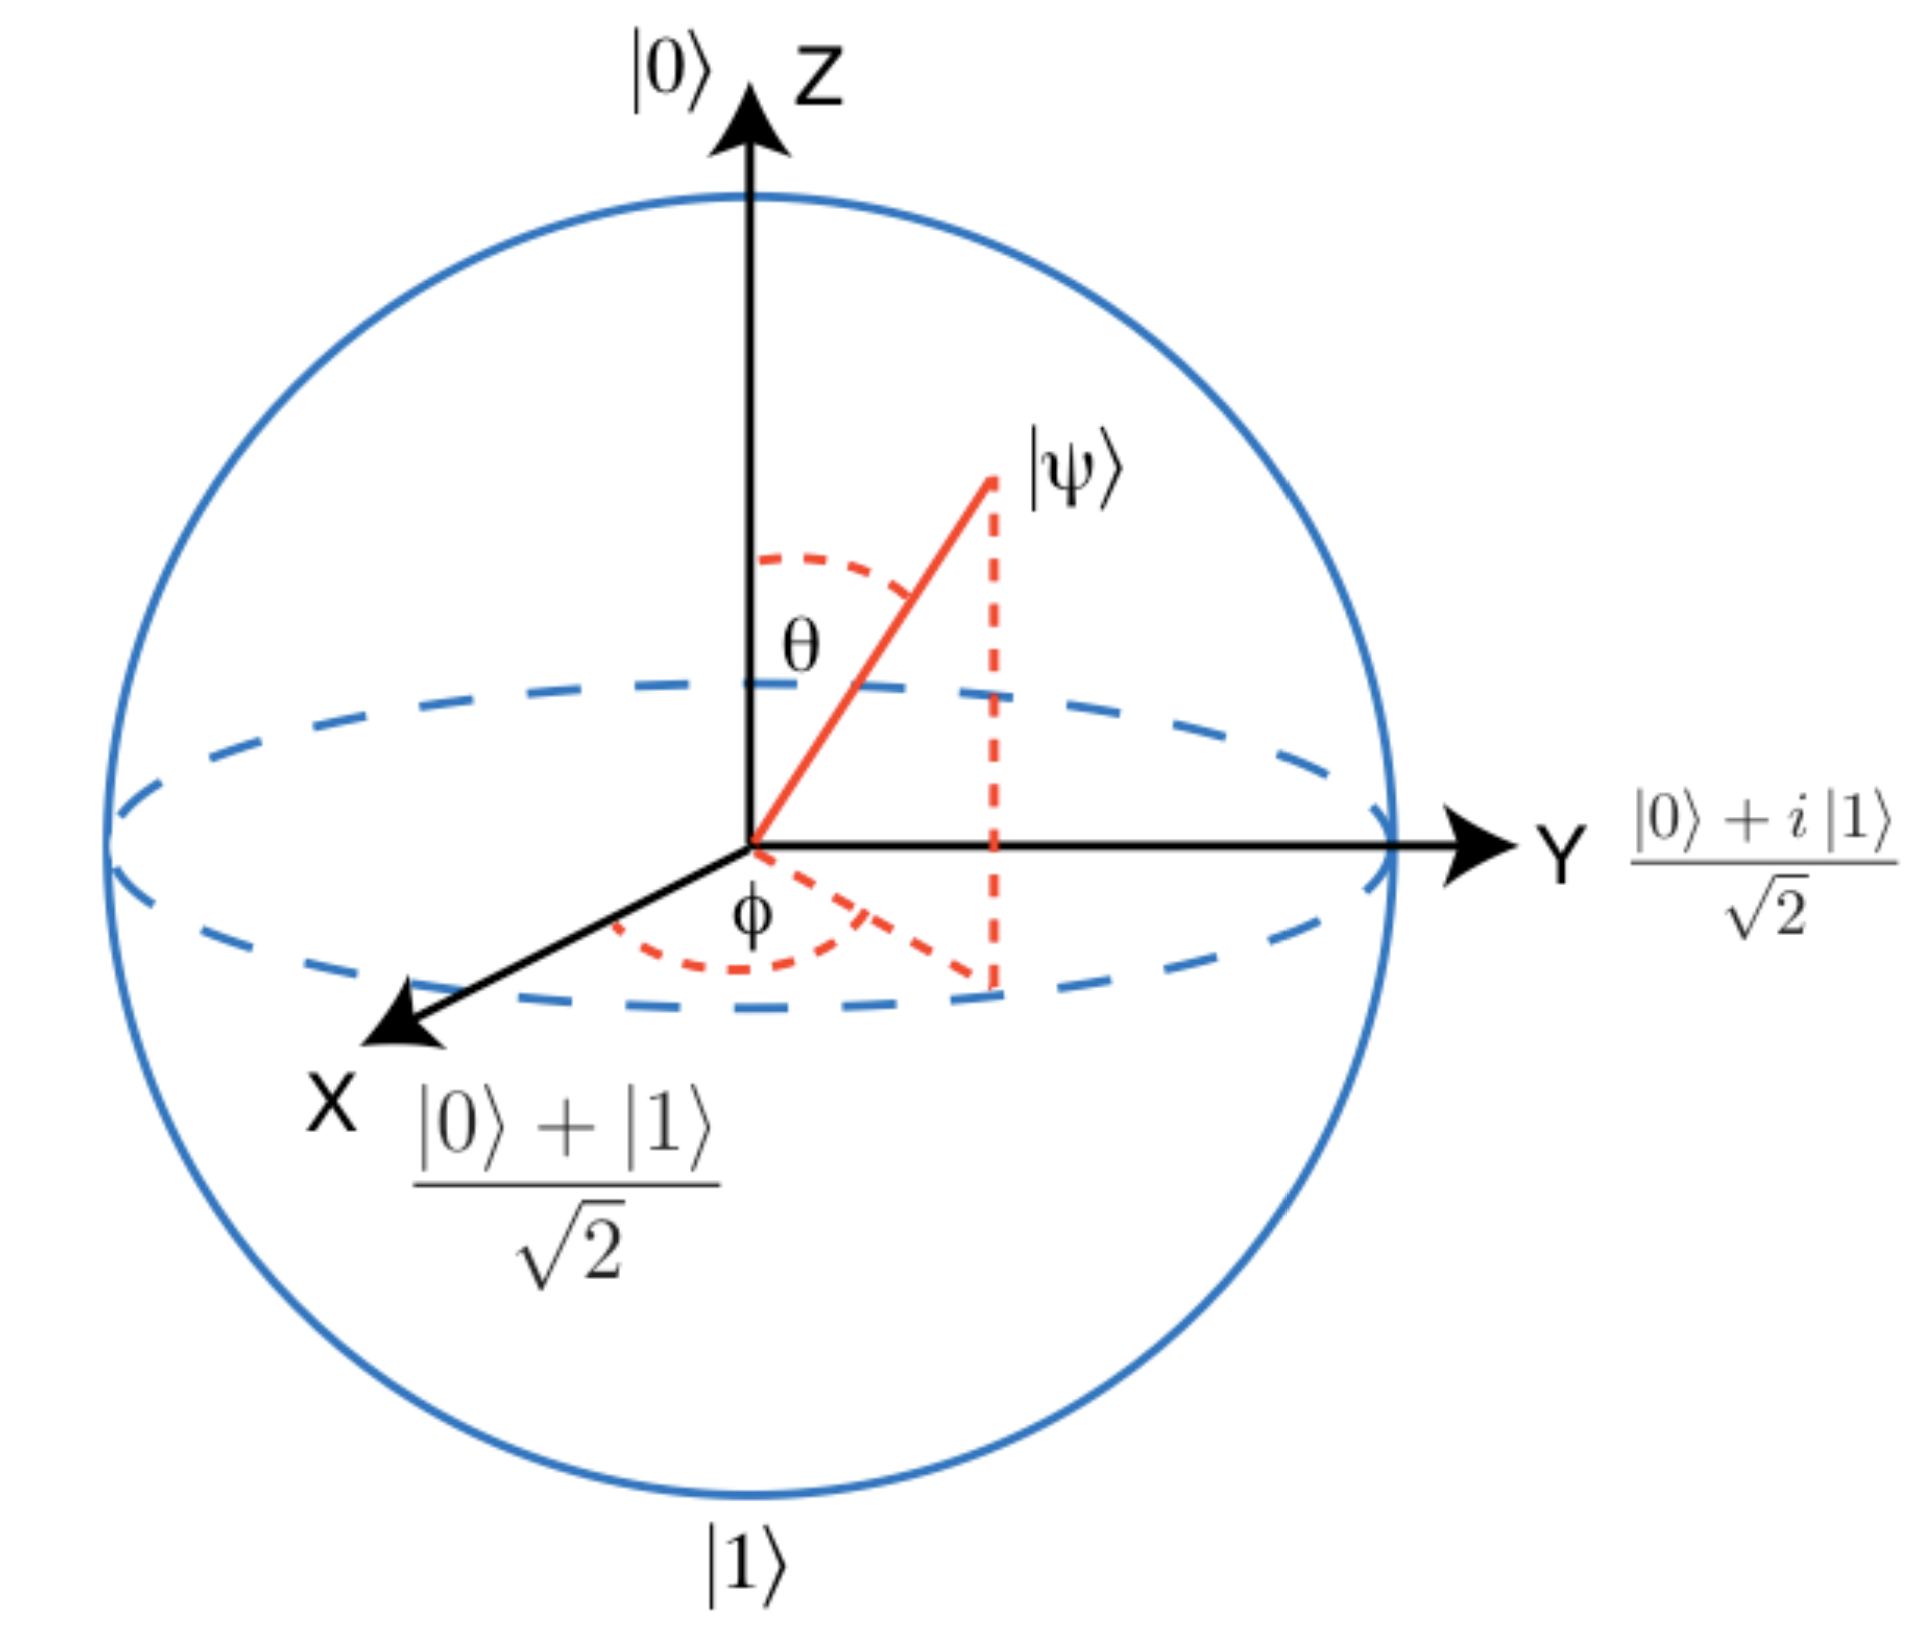
\includegraphics[width=0.55\textwidth]{figures/Bloch sphere.png}
  \caption{Geometrical representation of the Bloch sphere.}
\end{figure} \\
A property of qubits, as stated in Chapter \ref{Quantum computational chemistry}, is that if we want to process more than one of them, then a vector of the composite system can be expressed as the tensor product of all the basis states of the Hilbert spaces of the individual systems and the dimension of the composite system basis is the product of the dimensions of the individual systems. This also derives naturally from the first postulate of quantum mechanics. \\
As an example, if $\{ |0\rangle, |1\rangle \}$ is a basis for system A and system B, then the composite system AB can be expressed as
\begin{equation}
    |\Psi\rangle_{AB} = |\psi\rangle_A \otimes |\psi\rangle_B = \alpha |00\rangle + \beta |01\rangle + \gamma |10\rangle + \delta |11\rangle,
\end{equation}
where $\alpha, \beta, \gamma$ and $\delta$ are correctly defined to mantain the normalization of the vector, and the dimension of system AB is
\begin{equation}
    dim(AB) = dim(A) \cdot dim(B) = 2 \cdot 2 = 4.
\end{equation}
Again it is easy to see that for an N-qubits system the state is
\begin{equation}
    |\Psi\rangle = \frac{1}{\sqrt{2^N}} \sum_{x = 0}^{2^N - 1} |x\rangle,
\end{equation}
where $x$ is a string of binary numbers and the dimension of the system is
\begin{equation}
    dim(S_{1,2,...,N}) = dim(S_1) \cdot dim(S_2) \cdot ... \cdot dim(S_N) = 2 \cdot 2 \cdot ... \cdot 2 = 2^N.
\end{equation}
Here we described qubits as a coherent superposition of pure states. Coherence is essential for a qubit to be in such a state. If interactions, quantum noise and decoherence take place, it is possible to put the qubit in a mixed state, a statistical combination or 'incoherent mixture' of different pure states and that makes it hard to retrieve the correct computational states we were processing. Mixed states can be described with the so-called density matrix $\rho$ defined as
\begin{equation}
    \rho = \sum_i p_i |\psi_i\rangle \langle\psi_i|,
\end{equation}
where $p_i$ is the probability that the system is in state $|\psi_i\rangle$. These states are represented by points inside the Bloch sphere. A mixed qubit state has three degrees of freedom: the angles $\phi$ and $\theta$ and the length $r$ of the vector that represents the mixed state. It describes a real system that is evolving within a dynamical environment, which constantly interacts with the system. \\
This leads us to a more general definition: a 'physical' qubit is a physical device that behaves as a two-state quantum system, used as a component of a computer system. A 'logical' qubit is a physical (error-corrected) or abstract qubit that performs as specified in a quantum algorithm or quantum circuit subject to unitary transformations and has a long enough coherence time to be usable by quantum logic gates, which we will explore later. \\
This is an important distinction to keep in mind when one describes quantum algorithms, because, since quantum systems are hard to control, it is also hard to keep them isolated from the environment, thus, theoretically one can work only with logical qubits, but to complete the computation it is necessary to describe also the real system, i.e. the hardware, where the algorithm can be run.

\subsection{Quantum gates}
Quantum gates are derived from the second postulate of quantum mechanics, that is: every physical quantity is described as a Hermitian operator, i.e. a linear and unitary operator, acting in the state space $\mathcal{H}$. This operator is an observable, meaning that its eigenvectors form a basis for $\mathcal{H}$. \\
For this reason quantum gates are invertible and reversible, whereas classic gates are irreversible unless one takes into account trash bits. \\
Hermitian operators belongs to the unitary group $U(2)$ and can be represented by $2 \times 2$ matrices. \\
\\
There are two types of quantum gates: single-qubit gates and multiple-qubits gates. \\
The most important single-qubit gates are:
\begin{itemize}
    \item \textbf{Pauli gates ($X$, $Y$ and $Z$)} \\
    These three gates correspond to the Pauli operators and are represented with the three Pauli matrices, which define the spin observable of spin-$\frac{1}{2}$ particles.
    \begin{equation}
        X = \sigma_x = NOT = \left( \begin{array}{cc} 0 & 1 \\
                                                1 & 0 \end{array} \right)
    \end{equation}
    \begin{equation}
        Y = \sigma_y = \left( \begin{array}{cc} 0 & -i \\
                                                i & 0 \end{array} \right)
    \end{equation}
    \begin{equation}
        Z = \sigma_z = \left( \begin{array}{cc} 1 & 0 \\
                                                0 & -1 \end{array} \right)
    \end{equation}
    The $X$ gate is the quantum equivalent of the $NOT$ gate for classical computers with respect to the computational basis, which distinguishes the $z$ axis on the Bloch sphere. It is sometimes called 'bit-flip' as it swaps the two pure states,
    \begin{equation}
        X|\psi\rangle = X (\alpha |0\rangle + \beta |1\rangle) = \alpha |1\rangle + \beta |0\rangle.
    \end{equation}
    The eigenvectors of the $Z$ gate are the vectors that form the computational basis,
    \begin{equation}
        Z|0\rangle = |0\rangle, \ Z|1\rangle = -|1\rangle.
    \end{equation}
    The $Z$ gate is also called 'phase-flip'. \\
    Each gates performs a rotation of an angle $\pi$ around the corresponding axis on the Bloch sphere.
    
    \item \textbf{Hadamard gate ($H$)}
    \begin{equation}
        H = \frac1{\sqrt2} \left( \begin{array}{cc} 1 & 1 \\
                                                    1 & -1 \end{array} \right)
    \end{equation}
    This is the transformation that creates a superposition of pure states,
    \begin{equation}
        H|0\rangle = \frac{1}{\sqrt{2}} (|0\rangle + |1\rangle) = |+\rangle,
    \end{equation}
    \begin{equation}
        H|1\rangle = \frac{1}{\sqrt{2}} (|0\rangle - |1\rangle) = |-\rangle.
    \end{equation}
    
    \item \textbf{Rotation gates ($R_x$, $R_y$ and $R_z$)} \\
    The rotation operator gates are the angle rotation matrices in three cartesian axes of SO(3).
    \begin{equation}
        R_x(\theta) = e^{-iX\frac{\theta}{2}} = \left( \begin{array}{cc} cos\frac{\theta}{2} & -i \ sin\frac{\theta}{2} \\
        -i \ sin\frac{\theta}{2} & cos\frac{\theta}{2} \end{array} \right)
    \end{equation}
    \begin{equation}
        R_y(\theta) = e^{-iY\frac{\theta}{2}} = \left( \begin{array}{cc} cos\frac{\theta}{2} & - sin\frac{\theta}{2} \\
        sin\frac{\theta}{2} & cos\frac{\theta}{2} \end{array} \right)
    \end{equation}
    \begin{equation}
        R_z(\theta) = e^{-iZ\frac{\theta}{2}} = \left( \begin{array}{cc} e^{-i\frac{\theta}{2}} & 0 \\
        0 & e^{i\frac{\theta}{2}} \end{array} \right)
    \end{equation}
    A more general form is
    \begin{equation}
        R_{\hat{n}}(\theta) = e^{-i\frac{\theta}{2}\hat{n} \cdot \vec{\sigma}} = cos\frac{\theta}{2} \ I - i sin\frac{\theta}{2} \ \hat{n} \cdot \vec{\sigma},
    \end{equation}
    where $I$ is the identity operator.
    
    \item \textbf{Phase shift gates (P)}
    \begin{equation}
        P(\varphi) = \left( \begin{array}{cc} 1 & 0 \\
                                              0 & e^{i\varphi} \end{array} \right),
    \end{equation}
    where $\varphi$ is the phase shift with the period $2\pi$. \\
    The probability of measuring a $|0\rangle$ or $|1\rangle$ is unchanged after applying this gate, however it modifies the phase of the quantum state. This is equivalent to tracing a horizontal circle (a line of latitude), or a rotation along the $z$-axis on the Bloch sphere by $\varphi$ radians. \\
    Some common examples are:
    \begin{equation}
        P(\pi) = Z = \left( \begin{array}{cc} 1 & 0 \\
                                              0 & -1 \end{array} \right)
    \end{equation}
    \begin{equation}
        P\left(\frac{\pi}{2}\right) = S = \sqrt{Z} = \left( \begin{array}{cc} 1 & 0 \\
                                                                0 & i \end{array} \right)
    \end{equation}
    \begin{equation}
        P\left(\frac{\pi}{4}\right) = T = \sqrt{S} = \left( \begin{array}{cc} 1 & 0 \\
                                                        0 & e^{\frac{\pi}{4}} \end{array} \right)
    \end{equation}
    The gate performs a phase rotation in U(1) along the specified basis state.
\end{itemize}
Multiple-qubits gates transform states from multiple qubits at once, as long as the number of input qubits is equal to the number of output qubits, to preserve the unity property of quantum gates. \\
The most important ones are:
\begin{itemize}
    \item \textbf{Controlled gates ($CU$)} \\
    If $U$ is a gate that operates on a single qubit with matrix representation
    \begin{equation}
        U = \left( \begin{array}{cc} u_{00} & u_{01} \\
                                     u_{10} & u_{11} \end{array} \right),
    \end{equation}
    then the controlled-$U$ gate operates on two qubits in such a way that the first qubit serves as a control and the second is the target of the operator $U$,
    \begin{equation}
        CU = \left( \begin{array}{cccc} 1 & 0 & 0 & 0 \\
                                        0 & 1 & 0 & 0 \\
                                        0 & 0 & u_{00} & u_{01} \\
                                        0 & 0 & u_{10} & u_{11} \end{array} \right)
    \end{equation}
    An important example is $U = X$, this gate is also called Controlled-$NOT$ or $CNOT$ gate,
    \begin{equation}
        CNOT = \left( \begin{array}{cccc} 1 & 0 & 0 & 0 \\
                                          0 & 1 & 0 & 0 \\
                                          0 & 0 & 0 & 1 \\
                                          0 & 0 & 1 & 0 \end{array} \right),
    \end{equation}
    it performs the $NOT$ operation on the second qubit only when the first qubit is in state $|1\rangle$, and otherwise leaves it unchanged. For a comparison, it acts like a $XOR$ classical gate plus a trash bit to take account of reversibility. \\
    Another example is $U = P$
    \begin{equation}
        CP = \left( \begin{array}{cccc} 1 & 0 & 0 & 0 \\
                                        0 & 1 & 0 & 0 \\
                                        0 & 0 & 1 & 0 \\
                                        0 & 0 & 0 & e^{i\varphi} \end{array} \right).
    \end{equation}
    
    \item \textbf{Swap gate} \\
    The swap gate swaps the states of two qubits.
    \begin{equation}
        SWAP = \left( \begin{array}{cccc} 1 & 0 & 0 & 0 \\
                                          0 & 0 & 1 & 0 \\
                                          0 & 1 & 0 & 0 \\
                                          0 & 0 & 0 & 1 \end{array} \right)
    \end{equation}
    
    \item \textbf{Toffoli gate (TOFFOLI, CCNOT)}
    \begin{equation}
        TOFFOLI = CCNOT = \left( \begin{array}{cccccccc} 1 & 0 & 0 & 0 & 0 & 0 & 0 & 0 \\
                                                         0 & 1 & 0 & 0 & 0 & 0 & 0 & 0 \\
                                                         0 & 0 & 1 & 0 & 0 & 0 & 0 & 0 \\
                                                         0 & 0 & 0 & 1 & 0 & 0 & 0 & 0 \\
                                                         0 & 0 & 0 & 0 & 1 & 0 & 0 & 0 \\
                                                         0 & 0 & 0 & 0 & 0 & 1 & 0 & 0 \\
                                                         0 & 0 & 0 & 0 & 0 & 0 & 0 & 1 \\
                                                         0 & 0 & 0 & 0 & 0 & 0 & 1 & 0 \end{array} \right)
    \end{equation}
    If the first two bits are in the state $|1\rangle$ it applies a $X$ gate on the third bit, else it does nothing. The Toffoli gate is an example of a $CCU$, controlled-controlled unitary gate.
    
    \item \textbf{n-times-controlled gate ($C^n(U)$)} \\
    This the generalization of the controlled and the controlled-controlled gates for any unitary gate $U$.
    \begin{equation}
        C^n(U) = \left( \begin{array} {ccccc} 1 & 0 & ... & 0 & 0 \\
                                             0 & 1 & ... & 0 & 0 \\
                                             . & . & . & . & . \\
                                             0 & 0 & ... & u_{00} & u_{01} \\
                                             0 & 0 & ... & u_{10} & u_{11} \end{array} \right)
    \end{equation}
    
\end{itemize}
\begin{figure}[ht]
  \centering
  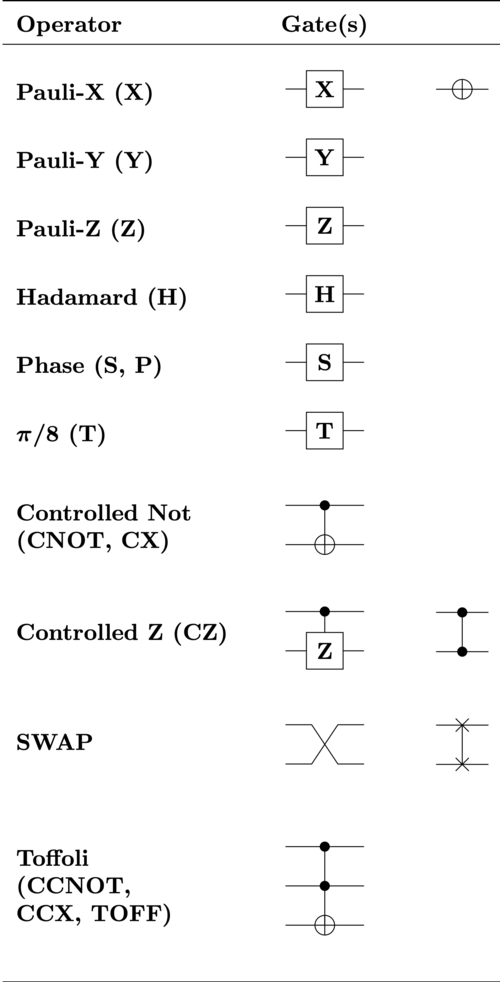
\includegraphics[width=0.45\textwidth]{figures/Quantum_Logic_Gates.png}
  \caption{Summary of the main quantum gates and their representation on a circuit.}
\end{figure}

\subsection{Measurement}
Measurement, also called observation, is an irreversible process and therefore not a quantum gate, because it assigns the observed quantum state to a single value. It takes a quantum state and projects it to one of the basis vectors with a likelihood equal to the square of the vector's length along that basis vector. This is known as the 'Born rule' or the third postulate of quantum mechanics and appears as a stochastic non-reversible operation as it probabilistically sets the quantum state equal to the basis vector that represents the measured state. At the instant of measurement, the state is said to 'collapse' to the definite single value that was measured. Why and how, or even if the quantum state collapses at measurement, is called the measurement problem. \\
Measuring a single qubit, whose quantum state is represented by the vector in eq. (\ref{qubit}), will result in $|0\rangle$ with probability $|\alpha|^{2}$, and in $|1\rangle$ with probability $|\beta|^2$. \\
If we take a quantum state $|\Psi \rangle$ that spans a register, i.e. a collection of $N$ qubits, this can be measured to $2^{N}$ distinct states, similar to how a register of $n$ classical bits can hold $2^{N}$ distinct states. Unlike with the bits of classical computers, quantum states can have non-zero probability amplitudes in multiple measurable values simultaneously. This is called superposition. \\
As mentioned before, the sum of all probabilities for all outcomes must always be equal to 1. \\
We can formally define the measurement operation as the application of the operator $M_m$
\begin{equation}
    |\psi\rangle \rightarrow \frac{M_m |\psi\rangle}{\sqrt{\langle\psi|M_m^\dagger M_m|\psi\rangle}},
\end{equation}
and the probability of finding the eigenvalue $a_m$ is
\begin{equation}
    \mathbb{P}(a_m) = |\langle a_m|\psi \rangle|^2.
\end{equation}
\begin{figure}[ht]
  \centering
  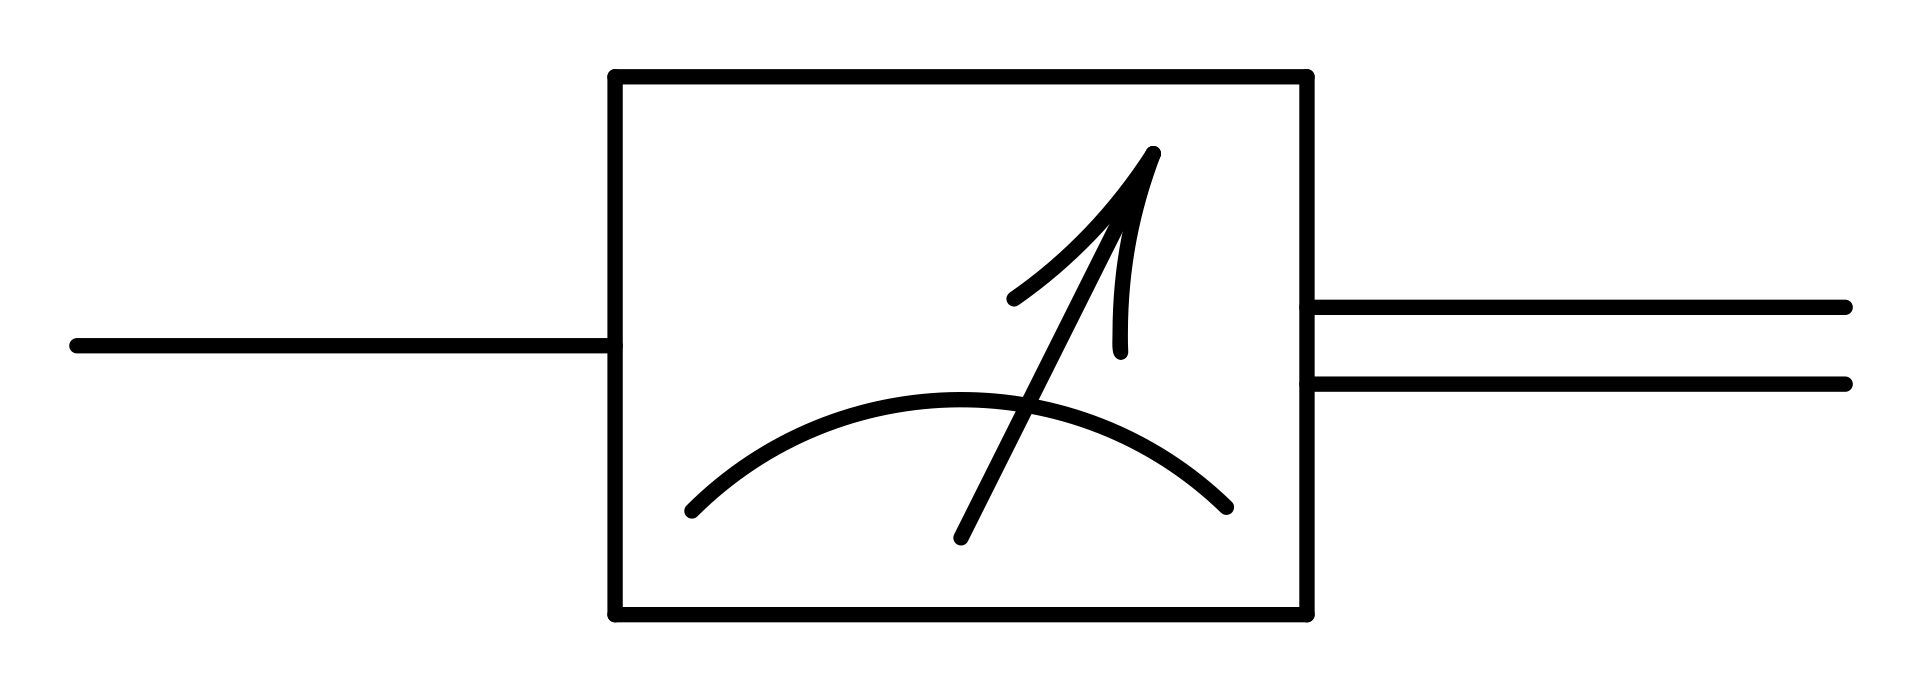
\includegraphics[width=0.3\textwidth]{figures/Measurement.png}
  \caption{Representation of the measurement process in a circuit.}
\end{figure} \\
Generally the computational basis $\{ |0\rangle,|1\rangle \}$ is used to project the states of the qubits, but different basis can be used, such as the basis $\{ |+\rangle,|-\rangle \}$.

\section{Important results}
\subsection{Set of universal quantum gates}
A small set of classical gates, e.g. $AND+OR+NOT$ or $NAND+FANOUT$, can be used to compute an arbitrary classical function. We say that such a set of gates is universal for classical computation. \\
Similarly in quantum computing, a set of universal quantum gates is any set of gates to which any possible operation on a quantum computer can be reduced, that is, any other unitary operation can be expressed as a finite sequence of gates from the set. Technically, this is impossible with anything less than an uncountable set of gates since the number of possible quantum gates is uncountable, whereas the number of finite sequences from a finite set is countable. To solve this problem, we only require that any quantum operation can be approximated by a sequence of gates from this finite set. \\
The rotation operators $R_x$, $R_y$, $R_z$, the phase shift $P$ and the $CNOT$ gates form a universal set of quantum gates. \\
A common universal gate set is the Clifford + $T$ gates set, which is composed of the $CNOT$, $H$, $S$ and $T$ gates. \\
The last statement can be demonstrated rigorously by decomposing generic unitary gates into single-qubit gates and $CNOT$ gates and then by approximating single-qubit gates with products of $H$ and $T$ gates. The $P$ gates are needed to make the approximation fault-tolerantly, i.e. during the computation the states are encoded in a way that prevent interactions, quantum noise and decoherence to produce errors and lose information \cite{Nielsen2010Dec}. \\
\\
This knowledge allows us to decompose every circuit in a simpler one that contains only this set of gates. This is useful especially for highly-correlated circuits, i.e. circuits with many multiple-qubits gates, that are complicated to implement due to the difficulty of controlling interactions between individual qubits with high precision. \\
A simple example is the decomposition of the $X$ and $Z$ gates in a sequence of $H$ and $S$ gates,
\begin{equation}
    Z = \left( \begin{array}{cc} 1 & 0 \\
                                 0 & -1 \end{array} \right)
      = \left( \begin{array}{cc} 1 & 0 \\
                                 0 & i \end{array} \right)
        \left( \begin{array}{cc} 1 & 0 \\
                                 0 & i \end{array} \right)
      = SS,
\end{equation}
\begin{equation}
    X = \left( \begin{array}{cc} 0 & 1 \\
                                 1 & 0 \end{array} \right)
      = HZH = HSSH.
\end{equation}
Unfortunately, the decomposition of a generic unitary transformation on $N$ qubits through a small set of elementary gates is generally hard, meaning that there is no efficient way to do it \cite{Motta2021Dec}. To see this, suppose we have $g$ different types of gates available, and each gate works on at most $f$ input qubits. These numbers, $f$ and $g$, are fixed by the computing hardware we have available, and may be considered to be constants. Suppose we have a quantum circuit containing $m$ gates, starting from the computational basis state $|0\rangle^{\otimes N}$. For any particular gate in the circuit there are therefore at most $\left[ {\begin{array}{c} N \\ f \end{array} } \right]^g = O(N^{fgm})$ possible choices. It follows that at most $O(N^{fgm})$ different states may be computed using $m$ gates, meaning there are unitary operations requiring exponentially many operations. \\
Thus, to within a polynomial factor the construction for universality is optimal. Unfortunately, it does not address the problem of determining which families of unitary operations can be computed efficiently in the quantum circuits model. \\

\subsection{Gottesman-Knill theorem}
A very important result in quantum information is the Gottesman-Knill theorem. It provides a connection between quantum and classical computing in terms of efficient computation, which, as we already saw, is a fundamental topic throughout all of computer science. \\
\\
Generally we say that a quantum computation can be efficiently simulated classically in the 'strong' sense, if it is possible to evaluate the function $\alpha \in \{0,1\}^S \rightarrow \pi(\alpha)$ up to $M$ digits in $poly(M,N)$ time on a classical computer, where $N$ is the number of qubits, $\alpha$ is the measurement outcome bit string, $S$ is the subset of qubits measured and $\pi(\alpha)$ is the probability that the outcome $\alpha$ occurs, given by
\begin{equation}
    \pi(\alpha) = \langle0|^{\otimes N}U^{\dagger}|\alpha\rangle\langle\alpha|^S U|0\rangle^{\otimes N}.
\end{equation}
Furthermore, we say that the quantum computation can be efficiently simulated classically in the 'weak' sense if it is possible to sample once from the probability distribution $\{ \pi(\alpha) \}$ in $poly(N)$ time on a classical computer. \\
\\
The Gottesman-Knill theorem states:
\begin{quote}
    \textit{Every uniform family of Clifford circuits, when applied to the input state $|0\rangle^{\otimes N}$ and when followed by a measurement of an arbitrary subset of qubits in the computational basis, can be efficiently simulated classically in the strong sense.}
\end{quote}
This can be proved using stabilizer operations, i.e. operations that leave the state unchanged. One can build a generic state by using only Clifford gates, then decompose them in Pauli gates and show that they are stabilizer operations for this generic state. Using this stabilizer description it can then be shown that the measurement outcomes of computational basis measurements can efficiently be computed on a classical computer, hence showing that Clifford circuits can be efficiently simulated classically in the strong sense. \\
\\
The theorem leads to the conclusion that any quantum circuit which is composed of only $H$, $P$ and $CNOT$ gates can not provide any speedup with respect to classical computation. \\
This result exhibits some rather remarkable and sometimes puzzling features, not all of which are fully understood. For example, even though they are efficiently classically simulatable, Clifford circuits can generate a high degree of entanglement. This very feature raises doubts about the often-quoted statement that “entanglement is responsible for the quantum computational speedup”. In particular, it highlights that, while the presence of certain types of entanglement in a quantum computation is provably necessary to disallow efficient classical simulation, it is certainly not sufficient \cite{Nest2008Nov}. \\
Nevertheless, supplementing Clifford operations with essentially any non-Clifford gate immediately yields the full quantum computational model, as we have shown before.

\subsection{Quantum computational complexity}
There is considerable interest in developing a theory of quantum computational complexity, and relating it to classical computational complexity theory, which will doubtlessly represent an enormously fruitful direction for future researchers. Here we present an introductory discussion. \\
In classical computation we can define the $\bf{PSPACE}$ as the  class of decision problems which can be solved on a Turing machine using space polynomial in the problem size and an arbitrary amount of time. \\
$\bf{BQP}$ is an essentially quantum complexity class consisting of those decision problems that can be solved with bounded probability of error using a polynomial size quantum circuit. \\
One of the most significant results in quantum computational complexity is that $\bf{BQP} \subseteq \bf{PSPACE}$. It is clear that $\bf{BPP} \subseteq \bf{BQP}$, where $\bf{BPP}$ is the classical complexity class of decision problems which can be solved with bounded probability of error using polynomial time on a classical Turing machine. Thus we have the chain of inclusions $\bf{BPP} \subseteq \bf{BQP} \subseteq \bf{PSPACE}$. Proving that $\bf{BQP} \neq \bf{BPP}$, i.e. quantum computers are more powerful than classical computers, will therefore imply that $\bf{BPP} \neq \bf{PSPACE}$. However, it is not presently known whether this is true and proving it would represent a major breakthrough in computer science. \\
To prove that $\bf{BQP} \subseteq \bf{PSPACE}$ we do a computation involving $poly(n)$ gates and calculate the probability of ending up in a generic state. Given that the individual unitary gates appearing are operations such as $H$, $CNOT$ and so on, it is clear that the individual probabilities can be calculated to high accuracy using only polynomial space on a classical computer, and thus the total probability can be calculated using polynomial space. Of course, this algorithm is rather slow, since there are exponentially many terms which need to be calculated. However, only polynomially much space is consumed, and thus $\bf{BQP} \subseteq \bf{PSPACE}$ \cite{Nielsen2010Dec}. \\
Therefore, the class of problems solvable on a quantum computer with unlimited time and space resources is no larger than the class of problems solvable on a classical computer. Stated another way, this means that quantum computers do not violate the Church–Turing thesis that any algorithmic process can be simulated efficiently using a Turing machine. Of course, quantum computers may be much more efficient than their classical counterparts, thereby challenging the strong Church–Turing thesis that any algorithmic process can be simulated efficiently using a probabilistic Turing machine. \\
\\
In the context of quantum simulation for quantum chemistry the simulation of Hamiltonian dynamics resides in the $\bf{BQP}$ class, while 'hard' problems can be found in the quantum Merlin-Arthur class ($\bf{QMA}$). The latter is defined similarly to the $\bf{NP}$ class for classical computation, i.e. it comprises the problems where putative solutions can be verified but not computed in polynomial time on a quantum computer. Producing a putative solution means executing a quantum circuit giving access to a wave function $\ket{\Psi}$ and verifying a putative solution means executing a second quantum circuit to ensure that $\ket{\Psi}$ is actually a solution of the problem of interest. In the context of quantum simulation for quantum chemistry the most important $\bf{QMA}$ problem is the simulation of Hamiltonian eigenstates. However, there are a number of practical considerations to take into account. For example, the statements of computational complexity theory refer to exact solutions of the problem at hand, and experience indicates that approximate methods can deliver accurate results for certain problems, which calls for a systematic characterization of quantum algorithms for chemistry in both accuracy and computational cost across a variety of chemical problems \cite{Motta2021Dec}.

\subsection{Quantum Fourier transform}
Moving on to quantum algorithms we show one of the most important quantum routines used by many important algorithms, like Shor's algorithm and quantum phase estimation: the quantum Fourier transform (QFT). \\
It is the analogous to the discrete Fourier transform. It is a linear transformation with the following action on the basis states:
\begin{equation}
    |x\rangle \rightarrow \frac1{\sqrt{N}} \sum_{y=0}^{N-1} e^{2\pi i \frac{xy}{N}} |y\rangle.
\end{equation}
Equivalently, the action on an arbitrary state may be written as
\begin{equation}
    \sum_{j=0}^{N-1} x_j |j\rangle \rightarrow \sum_{k=0}^{N-1} y_k |k\rangle,
\end{equation}
where the amplitudes $y_k$ are the discrete Fourier transform of the amplitudes $x_j$. \\
Since it is a linear transformation, the QFT can be implemented as the dynamics for a quantum computer. \\
It is helpful to write the state $|x\rangle$ using the binary representation
\begin{equation}
    |x\rangle = x_1 x_2 ... x_n = x_1 2^{n-1} + x_2 2^{n-2} + ... + x_n 2^0
\end{equation}
and to write a binary fraction as
\begin{equation}
    \frac{x_l}{2} + \frac{x_{l+1}}{4} + ... + \frac{x_m}{2^{m-l+1}} = 0.x_lx_{l+1}...x_m.
\end{equation}
With a little algebra the QFT can be given the following useful 'product representation':
\begin{equation}
    |x_1,...,x_n\rangle \rightarrow \frac{ (|0\rangle + e^{2\pi i 0.x_n}) (|0\rangle + e^{2\pi i 0.x_{n-1}x_n}) ... (|0\rangle + e^{2\pi i 0.x_1x_2...x_n}) }{2^{n/2}}.
\end{equation}
This representation makes it easy to derive an efficient circuit for the quantum Fourier transform. Such a circuit is shown in Figure \ref{QFT circuit}. Swap gates at the end of the circuit are used to reverse the order of the qubits. The gate $UROT_k$ denotes the unitary transformation
\begin{equation}
    UROT_k = \left( \begin{array}{cc} 1 & 0 \\
                                   0 & e^{2\pi i/2^k} \end{array} \right),
\end{equation}
which is a phase gate where $\varphi$ is the primitive $2^k$-th of unity. In the circuit they appear in the controlled form.
\begin{figure}[ht]
  \centering
  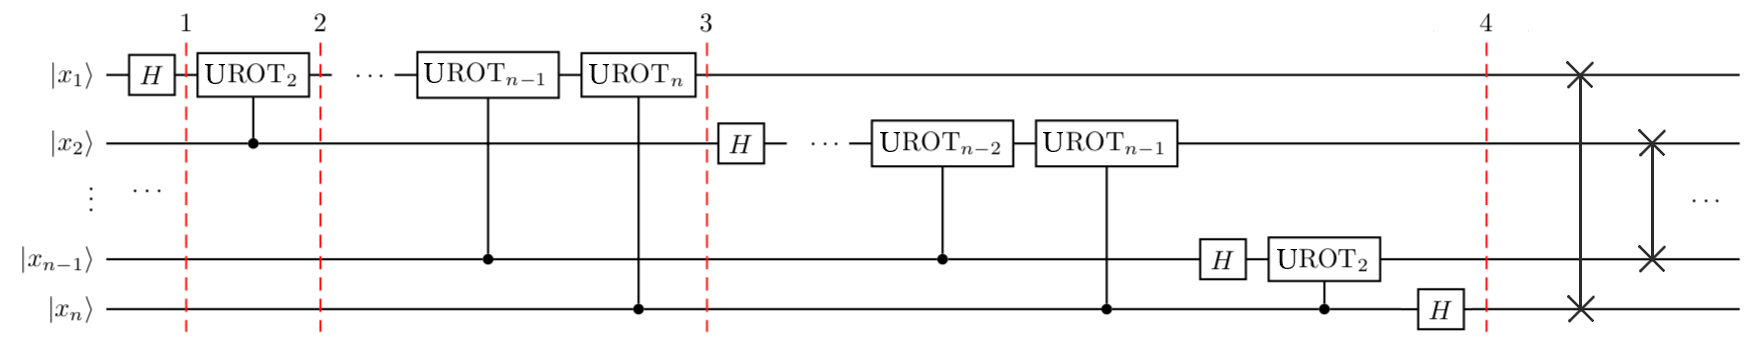
\includegraphics[width=\textwidth]{figures/QFT circuit 1.png}
  \caption{Circuit for the quantum Fourier transform.} \label{QFT circuit}
\end{figure} \\
This construction also proves that the quantum Fourier transform is unitary, since each gate in the circuit is unitary. \\
\\
How many gates does this circuit use? We start by doing a Hadamard gate and $n-1$ conditional rotations on the first qubit, a total of $n$ gates. This is followed by a Hadamard gate and $n-2$ conditional rotations on the second qubit, for a total of $n + (n-1)$ gates. Continuing in this way, we see that $n+(n-1)+...+1 = n(n+1)/2$ gates are required, plus the gates involved in the swaps. At most $n/2$ swaps are required, and each swap can be accomplished using three controlled-gates. Therefore, this circuit provides a $O(n^2)$ scaling algorithm for performing the QFT. \\
In contrast, the best classical algorithms for computing the discrete Fourier transform on $2n$ elements are algorithms such as the fast Fourier transform (FFT), which compute the discrete Fourier transform using $O(n2^n)$ gates. That is, it requires exponentially more operations to compute the Fourier transform on a classical computer than it does to implement the QFT on a quantum computer. \\
At face value this is an outstanding result, since the Fourier transform is a crucial step in so many real-world data processing applications. Can we use the QFT to speed up the computation of these Fourier transforms? Unfortunately, there is no known way to do this. The problem is that the amplitudes in a quantum computer cannot be directly accessed by measurement. Thus, there is no way of determining the Fourier transformed amplitudes of the original state. Worse still, there is in general no way to efficiently prepare the original state to be Fourier transformed. Thus, finding uses for the quantum Fourier transform turns out to be very subtle \cite{Nielsen2010Dec}.

\section{Quantum devices}
Experimental realization of quantum circuits, algorithms, and communication systems has proven extremely challenging. Here we explore some of the guiding principles and systems for physical implementation of quantum information processing devices and systems. \\
A quantum computer has to be well isolated in order to retain its quantum properties, but at the same time its qubits have to be accessible so that they can be manipulated to perform a computation and to read out the results. A realistic implementation must strike a delicate balance between these constraints, so that the relevant question is not how to build a quantum computer, but rather, how good a quantum computer can be built. \\
First of all, we must use systems with a two-state configuration to represent qubits, secondly, we must select a system in which they can be made to evolve as desired. Furthermore, we must be able to prepare qubits in some specified set of initial states and to measure the final output state of the system. \\
\begin{itemize}
    \item \textbf{Configurations} \\
    For the purpose of computation, the crucial realization is that the set of accessible states should be finite. It is generally desirable to have some aspect of symmetry dictate the finiteness of the state space, in order to minimize decoherence. For example, a spin-1/2 particle lives in a Hilbert space spanned by the $|\uparrow \ \rangle$ and $|\downarrow \ \rangle$ states, the spin state cannot be anything outside this two-dimensional space, and thus is a nearly ideal quantum bit when well isolated. A particle in a finite square well would make a mediocre quantum bit, because transitions from the bound states to the continuum of unbound states would be possible. These would lead to decoherence since they could destroy qubit superposition states. \\
    For single qubits the figure of merit is the minimum lifetime of arbitrary superposition states. A good measure, used for spin states and atomic systems, is $T_2$, the ‘transverse’ relaxation time of superposition states such as $\frac{|0\rangle + |1\rangle}{\sqrt{2}}$, while $T_1$ is the ‘longitudinal’ relaxation time of the higher energy $|1\rangle$ state, i.e. the classical state lifetime, which is usually longer than $T_2$.
    
    \item \textbf{Controllability} \\
    To perform quantum computation one must be able to control the Hamiltonian in order to effect an arbitrary selection from a universal family of unitary transformations. Unrecorded imperfections in unitary transforms can lead to decoherence. Similarly, the cumulative effect of systematic errors is decoherence when the information needed to be able to reverse them is lost. \\
    Two important figures of merit for unitary transforms are: the minimum achievable fidelity, $\mathcal{F}$, and the maximum time, $t_{op}$, required to perform elementary operations such as single spin rotations or a $CNOT$ gate.
    
    \item \textbf{State preparation} \\
    One of the most important requirements for being able to perform a useful computation, even classically, is to be able to prepare the desired input. Generally a computation starts with $N$ qubits in the state $|00...0\rangle$, but they may not stay there for very long due to thermal heating. Simply letting the system equilibrate establishes it in the thermal state, with the density matrix $\rho \approx e^{\mathcal{H}/k_bT}/\mathcal{Z}$. \\
    Two figures of merit are relevant to input state preparation are: the minimum fidelity with which the initial state can be prepared in a given state $\rho_{in}$ and the entropy of $\rho_{in}$, the latter is important because the input state is generally a pure state, with zero entropy.
    
    \item \textbf{Measurement} \\
    Let us think of measurement as a process of coupling one or more qubits to a classical system such that after some interval of time, the state of the qubits is indicated by the state of the classical system. Many difficulties with measurement can be imagined. Furthermore, projective measurements, sometimes called ‘strong’ measurements, are often difficult to implement. They require that the coupling between the quantum and classical systems be large, and switchable. Measurements should not occur when not desired; otherwise they can be a decoherence process. Surprisingly, however, strong measurements are not necessary; weak measurements which are performed continuously and never switched off, are usable for quantum computation. This is made possible by completing the computation in time short compared with the measurement coupling. \\
    A good figure of merit for measurement capability is the signal to noise ratio (SNR).
\end{itemize}
In the following we describe the main physical systems used to build quantum processor. \\
In Figure \ref{Core qubit technologies} are represented the most researched and mature qubit technologies.
\begin{figure}[ht]
  \centering
  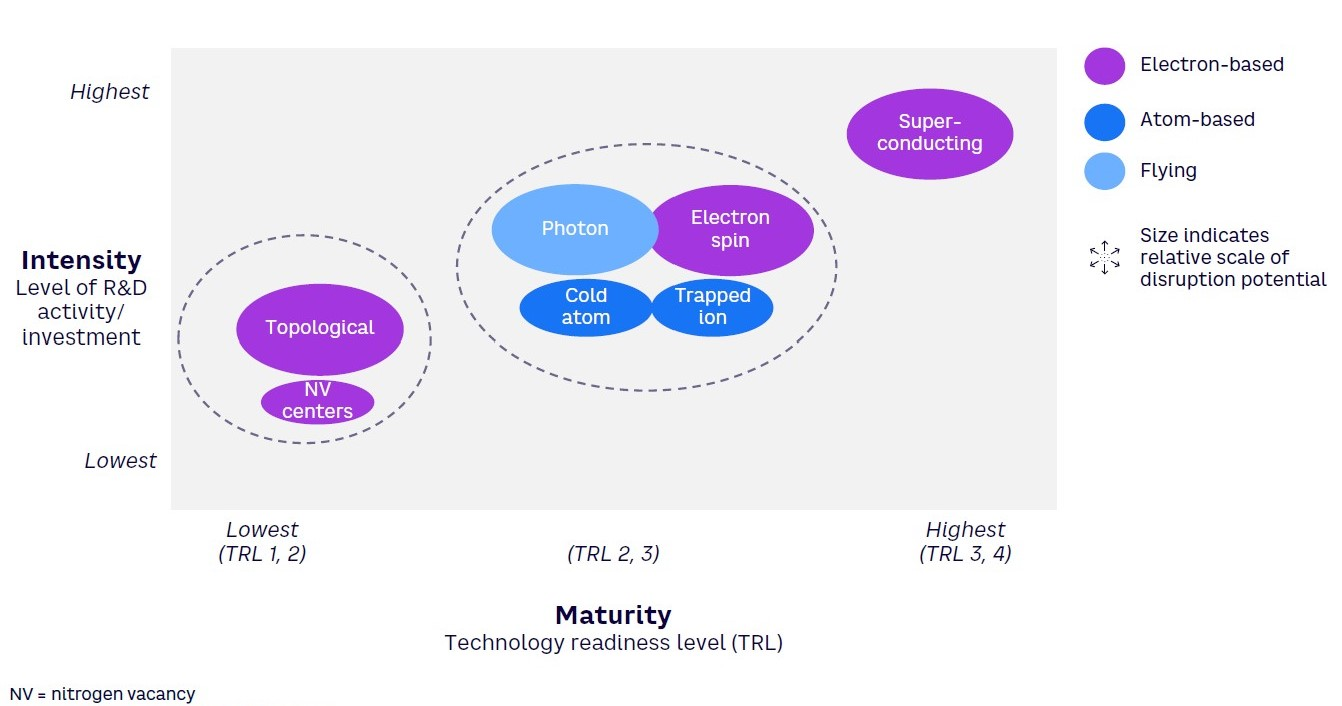
\includegraphics[width=\textwidth]{figures/Core qubit technologies.jpg}
  \caption{Core qubit technologies mapped by maturity, intensity and disruption potential \cite{BibEntry2022May}.} \label{Core qubit technologies}
\end{figure}

\subsection{Optical photons}
An attractive physical system for representing a quantum bit is the optical photon. It can be guided along long distances with low loss in optical fibers, delayed efficiently using phase shifters and combined using beamsplitters. \\
There are different ways to encode information in photonic qubits, for example path or polarization. The latter is defined as
\begin{equation}
    |0\rangle = |H\rangle, \ |1\rangle = |V\rangle,
\end{equation}
where $|H\rangle$ denotes horizontal polarization and $|V\rangle$ denotes vertical polarization. \\
Experimentally, the polarization of light can be manipulated with phase retarders or ‘wave plates'. These uniaxial, birefringent crystals introduce a polarization-dependent phase shift. Combining multiple wave plates facilitates the realization of every possible single-qubit gate
on polarization-encoded qubits. \\
Polarizing beam splitters can be used for the analysis of a polarization state. Combined with half-wave plates and quarter-wave plates they facilitate measurements in each possible direction on the Bloch sphere. \\
\\
Unfortunately, interaction between photons is difficult to achieve. In fact, because a nonlinear index of refraction is usually obtained by using a medium near an optical resonance, there is always some absorption associated with the nonlinearity. The standard process of creating entangled photons works probabilistically and with low efficiency and the quality of multi-photon states generated in a process are intrinsically limited due to noise caused by higher-order emissions. \\
Secondly, the development of efficient photonic two-qubits gates is of great importance. Although it has been shown that quantum computing is possible with only linear optics and photon detection, in practice these schemes become inefficient due to an enormous amount of required
ancilla photons. \\
Thirdly, current experiments are limited by the low detection efficiencies of avalanche photodiodes which are widely used in photonic quantum computing experiments. Much higher detection efficiencies can be obtained by employing superconducting transition-edge detectors or superconducting nanowire detectors. While poor time resolution of the former impedes their application in pulsed multi-photon experiments, the latter are ideally suited for this task \cite{BibEntry2016Jul}.

\subsection{Trapped ions}
Trapped ions are one approach to a large-scale quantum computer in which ions are confined and suspended in free space using electromagnetic fields. To achieve quantum computation with these, ion qubits are stored in the stable electronic states of each ion and quantum information is transferred through collective quantized motion of the ions in a shared trap. The manipulations made to these qubits are performed by lasers, where coupling is induced between qubit states for single qubit operations and between internal qubit states and external motional states for entanglement. \\
One can trap ions by using an apparatus known as a magneto-optical trap, or MOT for short. Magneto-optical traps rely on the principle of Doppler cooling. This is a mechanism that can be used to trap and slow the motion of atoms to cool a substance by operating on the principle of the Doppler shift experienced by the ion when hit by a laser photon. \\
To form a qubit one can produce hyperfine qubits, where the two states are two ground state hyperfine levels, or produce optical qubits, in which the two states are the ground state level and the excited level. Hyperfine qubits are quite long-lived, with experimental lifetimes often exceeding 10 minutes, and optical qubits, although shorter-lived, have lifetimes on the order of seconds, which is still long compared with logic gate operation time, which is on the order of microseconds for both types of qubits. \\
\\
We can prepare the qubits by optical pumping, in which a laser couples the ion to some excited states that can decay to one state which is not coupled to the laser. Eventually, after being excited enough times, the ion reaches a state in which it has no excited levels to couple to in the presence of that laser, and thus, the ion will remain in this state. After enough time essentially all of the ions will be in this state and therefore the qubits will be prepared. This preparation has extremely high fidelity, exceeding $99.9\%$. \\
To make a measurement we apply to the ion a laser that couples only one qubit state. We now have two cases for how the ion will collapse upon measurement: if the ion collapses to the state to which the laser is coupled then the laser excites the ion, resulting in the emission of a photon when the ion decays from the excited state, otherwise, if the ion collapses to the state to which the laser is not coupled then the laser does not excite the ion, and thus, no photons will be released. We can subsequently count the number of photons and determine the state of the qubit and, moreover, we can do so to very high accuracy, again exceeding $99.9\%$. \\
Regarding transformations, to implement single-qubit rotations for hyperfine qubits we can use magnetic dipole transitions or stimulated Raman transitions and for optical qubits we can achieve them via electric quadrupole transitions. For $CNOT$ gates there are various implementation, for example using $SWAP$ gates as well as controlled $Z$ gates. Such gates are generally no faster than one microsecond. These gates have a high fidelity, exceeding $99\%$ for each type of qubit. \\
\\
However, trapped-ion quantum computation is limited by the finite number of qubits that can be stored in each trap. Therefore, to achieve scalability, schemes have been introduced in which there are interconnected ion traps with storage and interaction regions. The qubits can thus be stored in the storage regions until they are needed for computation, at which point they can be shuttled to the interaction regions for manipulation. These qubits can turn corners at T junctions, which allows for a two-dimensional array trap design. Moreover, in the modern era of semiconductor fabrication, techniques have been employed to manufacture the ‘ion trap on a chip’, demonstrating the potential for scalability \cite{Bruzewicz2019Apr}.

\subsection{Superconducting circuits}
It is also possible to build quantum computers from superconducting electronic circuits. This research  is conducted by companies such as Google and IBM, e.g. the quantum processor Sycamore, designed by Google, uses 53 superconducting qubits. \\
In a superconductor the basic charge carriers are pairs of electrons, known as Cooper pairs, rather than the single electrons in a normal conductor. The total spin of a Cooper pair is an integer number, thus the Cooper pairs are bosons, i.e. electrons condense into Cooper pairs that form a single superfluid. \\
Superconducting qubits realize artificial atoms with engineered energy levels using the non-linearity of Josephson junctions and surrounding microwave circuitry. A Josephson junction consists of a thin layer of aluminium oxide, which is an insulator, sandwiched between two superconducting layers of aluminium, which becomes a superconductor when cooled below 1.2 K. The insulating layer is so thin (a few nanometres) that Cooper pairs can tunnel through it and couple the superconducting wave functions on either side of the barrier. \\
\\
The quantum dynamics of superconducting qubits follows that of a damped and driven anharmonic oscillator whose anharmonicity is controlled by choice of circuit parameters, e.g. linear capacitance and inductance of the Josephson junction. For experimental design and control practitioners draw from the Jaynes-Cummings model and its variants from cavity quantum electrodynamics (QED). Circuit quantum electrodynamics borrows the application of second quantized Hamiltonians from atomic optics via a standardized procedure for quantizing passive circuit. \\
The operational modes of superconducting qubits vary by their energy spectra, where non-linearity plays a role in realizing accessible and isolated states. If we consider the lowest two levels of the quantum harmonic oscillator to be the ground and excited states of a qubit, $|g\rangle$ and $|e\rangle$, the energies for the two states are separated by integer multiples of $\hbar\omega$. When we use an anharmonic oscillator the spacing between these two states is larger, further isolating the qubit states from the other states of the oscillator. An qubit built upon this system is also called a transmon. \\
An anharmonic oscillator-based superconducting qubit inherits its non-linearity from Josephson junctions, where the non-linearity is tunable through fabrication and microwave circuit design. This is because there are several phenomenological models for Josephson junctions. \\
The behaviour of the electron superfluid is completely determined by a single quantum wave function. The amplitude of this wave function determines the number of Cooper pairs, while the value of the phase is related to the supercurrent and any magnetic field that is present. \\
\\
The two primary types of superconducting qubit, the charge qubit and the flux qubit, are directly related to two variables: charge qubits are associated with the amplitude, while flux qubits are related to the phase. \\
For a flux qubit a standard circuit is composed by three Josephson junctions connected by superconducting aluminium leads to form a closed loop and uses an applied magnetic field, perpendicular to the loop, to drive the circuit by controlling the phase. When the magnetic flux through the loop, $\phi$, is equal to half the quantum of magnetic flux in a superconductor, the state with a zero phase difference around the loop ($|0\rangle$) has the same energy as the state with a $2\pi$ phase difference ($|1\rangle$). One of these states corresponds to a current circulating around the loop in the clockwise direction, while the other state corresponds to a current moving in the opposite direction \cite{Materise2017Aug}. \\
Measurements are made with a superconducting quantum interference device (SQUID). This device, which consists of two Josephson junctions in parallel, is the most sensitive magnetic-flux detector known. \\
If we shine a coherent state light with frequency $\omega_a$, i.e. the transmon frequency gap, on the cavity and phase $\phi$ at the position of the qubit, then the Hamiltonian for the artificial atom is
\begin{equation}
    H = \hbar \Omega_R (\sigma_x cos\phi + \sigma_y sin\phi),
\end{equation}
where $\Omega_R$ is called the Rabi frequency, which depends on the average electric field in the cavity and the size of the superconducting qubit. With this Hamiltonian we can implement a universal set of single-qubit gates since $\phi = 0$ implements an $X$-rotation and $\phi = \frac{\pi}{2}$ applies a $Y$-rotation. \\
As for multiple-qubits gates, an advantage of superconducting technology is the variety of options to connect qubits with each other. One of the best ways is via capacitative coupling, where we connect two transmons through a wire and coupling capacitor. We can form a Hamiltonian that allows to implement the two-qubits $iSWAP$ gate and if we combine this with $X$- and $Z$-rotations we can build a $CNOT$ gate, thus enabling universal quantum computation. \\
Nonetheless, there are still some technological challenges preventing superconducting qubits from scaling further. A glaring issue is that we need to keep the transmons at very low temperatures, which requires the use of large cryogenic devices known as dilution refrigerators. In the future other quantum technologies may bypass the use of low temperatures, but superconducting qubits may not be so lucky, since they are constrained by the laws of physics that allow for superconductivity. \\
Superconducting circuits are large compared to other quantum systems, so their interaction with the environment is difficult to control. As a consequence, the excited state lasts for about 1 micro-second before decaying back to the ground state. Current single-qubit gates are acceptable since they can be applied in a matter of nanoseconds, thanks to our ability to manufacture very small cavities. Problems arise, however, when we want to perform precise measurements of the qubit \cite{BibEntry2022Aug}. \\
\\
In Figures \ref{Advantages} and \ref{Disadvantages} are listed the main advantages and the disadvantages of trapped ions and superconducting qubits.
\begin{figure}[ht]
  \centering
  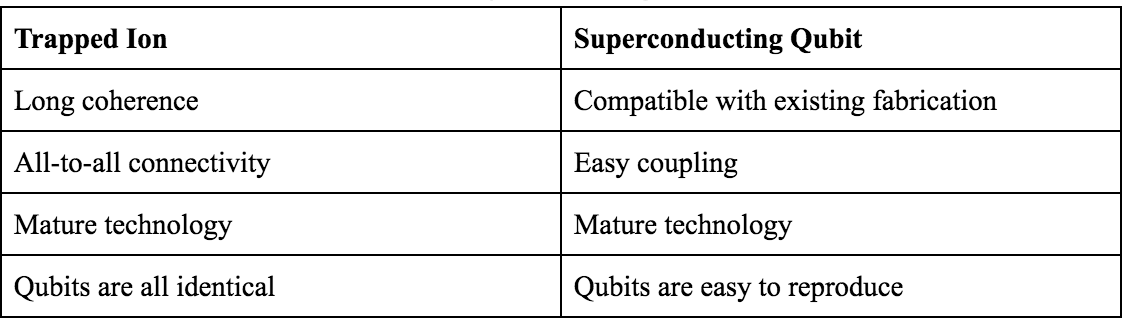
\includegraphics[width=0.9\textwidth]{figures/Advantages trapped ions vs superconducting.png}
  \caption{Advantages of trapped ions and superconducting qubits.} \label{Advantages}
\end{figure}
\begin{figure}[ht]
  \centering
  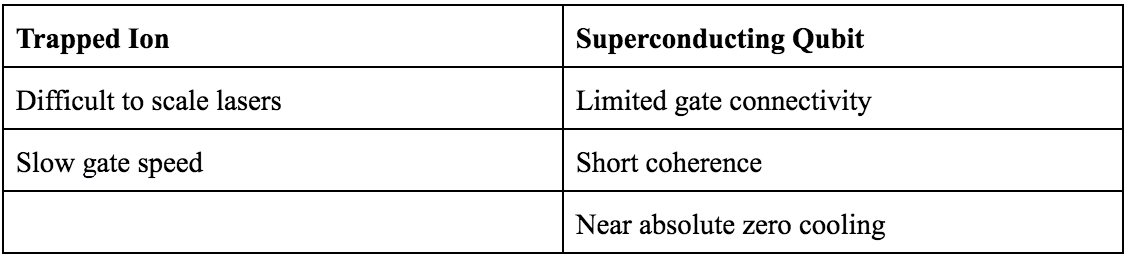
\includegraphics[width=0.9\textwidth]{figures/Disadvantages trapped ions vs superconducting.png}
  \caption{Disadvantages of trapped ions and superconducting qubits.} \label{Disadvantages}
\end{figure}